\chapter{图像分析的数据结构}
\section{图像数据表示的层次}
计算机视觉感知的目的是寻找输入图像与真实世界之间的关系。%
在从原始输入图像向模型的转换过程中,%
图像信息逐渐浓缩,%
使用的有关数据解释的语义知识也越来越多。%
在输入图像和模型之间,%
定义了若干层次的视觉信息表示,%
计算机视觉由如下的设计所组成。
\begin{itemize}
\item{中间表示(数据结构)}
\item{创建这些中间表示所用的算法和它们之间关系的导入}
\end{itemize}

\noindent{}这些表示可以分为四个层次:

最底层的表示,称为\textbf{\color{magenta}图标图像},%
由含有原始数据的图像组成,%
原始数据也就是像素亮度数据的整数矩阵,%
其中图像的预处理就发生在这个阶段。

第二层次的表示,称为\textbf{\color{magenta}分割图像},%
图像被分割为可能属于同一物体的区域。%
例如,多面体场景的图像分割的输出,%
或者是对应于边界的线段,%
或者是对应于表面的两维区域。%
在做图像分割时,%
了解具体的应用领域是有帮助的,%
这样就可以比较容易地处理噪声和与错误图像数据有关的其它问题。

第三层的表示,称为\textbf{\color{magenta}几何表示},%
保存2D和3D形状知识。%
形状的量化是非常困难的,%
但是也是十分重要的。%
在做普通而复杂的有关实际物体受光照和运动影响的模拟时,%
几何表示是有用的。

第四层的表示,称为\textbf{\color{magenta}关系模型},%
关系模型使我们能更有效地,%
并且在更高的抽象层次上处理数据。%
在这种处理中,一般需要使用一些有关解决问题的先验知识。%
通常会涉及人工智能(AI)技术,%
从图像中获得的信息可以表示成语义网络或框架。

\section{传统图像数据结构}
传统的图像数据结构有矩阵、链表、图、物体属性表、关系数据库,%
它们不仅对于直接表示的图像信息是重要的,%
而且还是更复杂的图像分层表示方法的基础。

\subsection{矩阵}
矩阵是低层图像表示的最普通的数据结构,%
矩阵元素是整型的数值,%
对应于采样栅格中的相应像素的亮度或其它属性。%
数据与矩阵元素的对应关系对于矩形栅格来说是显然的,%
对应于六边形栅格来说图像中的每个偶数行都要向右移动半个像素。

矩阵中的像素信息可以通过像素的坐标得到,%
坐标对应于行和列的标号,%
矩阵隐含着图像组成部分之间的\textbf{\color{magenta}空间关系}

用矩阵表示的特殊图像有:
\begin{itemize}
\item{\textbf{\color{magenta}二值图像}(仅有两个亮度级别的图像)用仅含有0和1的矩阵来表示。}
\item{\textbf{\color{magenta}多光谱图像}的信息可以用几个矩阵来表示,每个矩阵含有一个频带的图像。}
\item{\textbf{\color{magenta}分层图像数据结构}用不同分辨率的矩阵来获得。%
    图像的这种分层表示对于具有处理并行计算是非常方便的。}
\end{itemize}

矩阵中包含大量的图像数据,其中图像的全局信息是非常重要的。%
其中关于全局信息的直方图前面已经介绍过了,%
另一个重要的全局信息是\textbf{\color{magenta}共生矩阵(co-occurrence matrix)},%
它是亮度为$z$的像素$(i_{1},j_{1})$和亮度为$y$的像素$(i_{2},j_{2})$的具有空间关系的两个像素的概率估计。%
假设这个概率仅依赖于亮度$z$的像素和亮度$y$的像素之间的某个空间关系$r$,%
那么关于关系$r$的信息就记录在方形的共生矩阵$C_{r}$中,%
它的维度对应于图像的亮度级别数。%
为了减少矩阵$C_{r}$的数目,%
引进一些简化的假设,%
首先仅考虑直接的邻居,%
其次假定关系是对称的(没有行向)。%
计算图像$f(i,j)$的共生矩阵$C_{r}$算法如下:
\begin{algo}{关系$r$的共生矩阵}{关系$r$的共生矩阵}
  \textbf{
    \begin{itemize}
    \item{置$C_{r}(z,y)$ = 0,对于所有的$z,y\in[0,L]$,其中$L$是最大的亮度。}
    \item{对于图像中的所有像素$(i_{1},j_{1})$,找到与像素$(i_{1},j_{1})$有关系$r$的像素$(i_{2},j_{2})$,%
        做
        \begin{center}
          $C_{r}[f(i_{1},j_{1}),f(i_{2},j_{2})] = C_{r}[f(i_{1},j_{1}), f(i_{2},j_{2})]+1$
        \end{center}
      }
    \end{itemize}
}
\end{algo}

考虑共生矩阵的主要原因是其描述纹理的能力,%
这里我们给出详细的理解。

纹理特征是一种不依赖于颜色或亮度的反应图像中同质现象的视觉特征。%
习惯上将图像的局部不规则性和宏观上有规律的视觉特性称为纹理。%
它是所有物理表面共有的内在特征。%
正因为如此,纹理特征在基于内容的图像检索中得到了广泛的应用,%
用户可以通过提交包含有某种纹理特征的图像来查找含有显示纹理特征的其它图像。

基于灰度共生矩阵的纹理分析方法在很多方面的应用已经取得了很大的成功。%
但是人们并没有将它用于纹理图像分割,%
而是更多的应用于图像的分类。

\subsection{基于灰度共生矩阵的描述符}
由灰度共生矩阵(GLCM)获得的纹理特征主要是通过描述灰度值的空间分布来表征纹理的,%
具有计算简单等优点。%
其定义如下:\textbf{\color{magenta}灰度共生矩阵\dash 图像中相距为$d$的两个灰度像素同时出现的联合概率分布。}%
其意义为:\textbf{\color{magenta}共生矩阵方法用条件概率来反应纹理,%
  是相邻像素的灰度相关性的表现。}
\begin{gather}
  \begin{split}
    P_{c} &= p(i, j, d, 0^{\circ}) = \{(k, l), (m, n) \in G \times G |\\
    &|k-m|=d, l-n=0; f(k, 1) = i, f(m,n) = j\}
  \end{split}\\
  \begin{split}
    P_{c} &= p(i, j, d, 45^{\circ}) = \{(k, l), (m, n) \in G \times G |\\
    & k-m = l-n = d \text{或} k-m=l-n=-d; f(k, 1) = i, f(m,n) = j\}
  \end{split}\\
  \begin{split}
    P_{c} &= p(i, j, d, 90^{\circ}) = \{(k, l), (m, n) \in G \times G |\\
    & k-m = 0,  |l-n| = d; f(k, 1) = i, f(m,n) = j\}
  \end{split}\\
  \begin{split}
    P_{c} &= p(i, j, d, 135^{\circ}) = \{(k, l), (m, n) \in G \times G |\\
    & k-m = d, l-n = -d \text{或} k-m= -d, l-n=d; f(k, 1) = i, f(m,n) = j\}
  \end{split}
\end{gather}
\begin{figure}[hbpt]
  \centering
  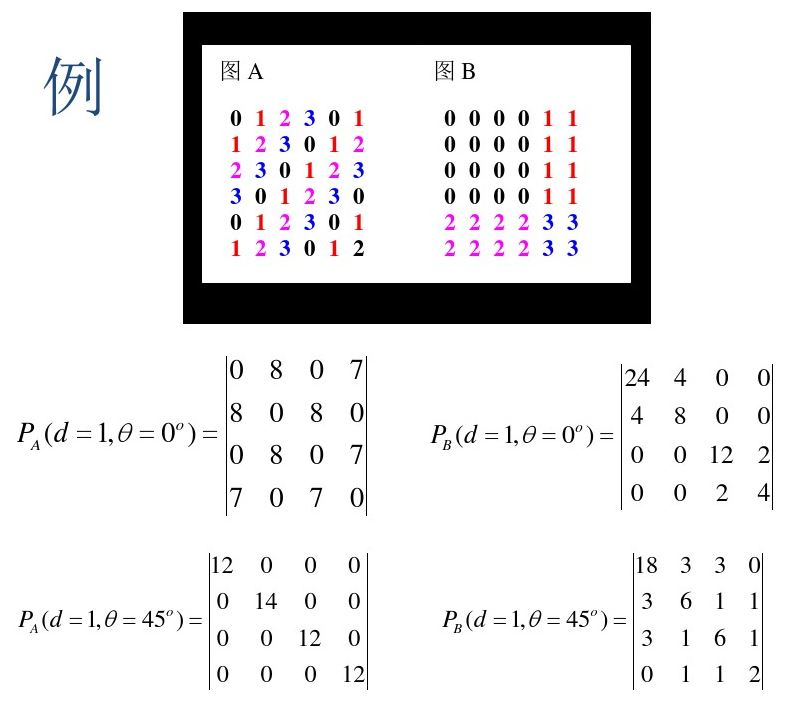
\includegraphics[width=0.8\textwidth]{图像分析的数据结构/Figures/共生矩阵例子}
\end{figure}

\begin{figure}[hbpt]
  \centering
  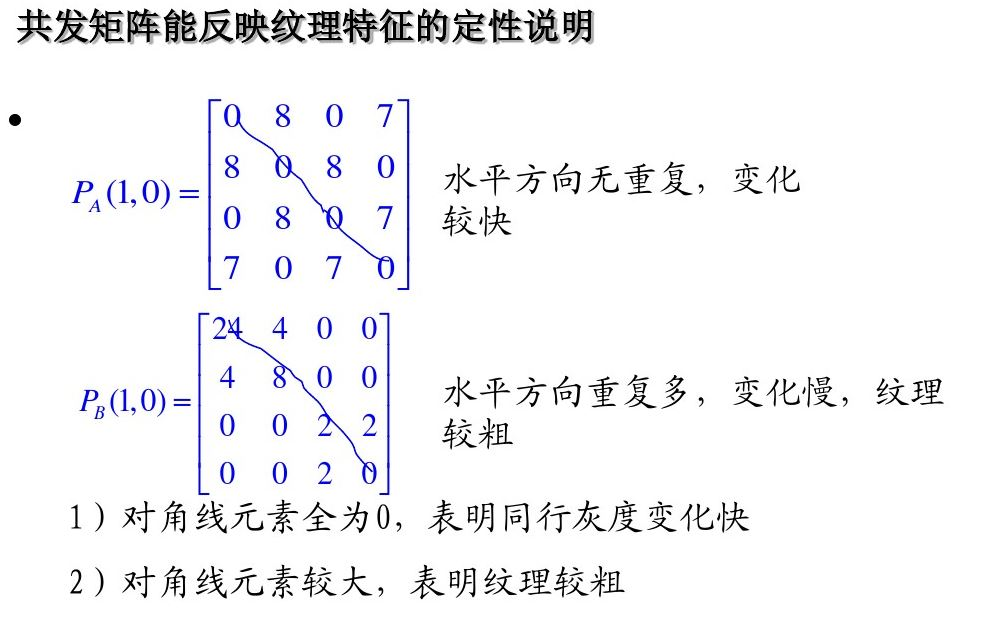
\includegraphics[width=0.8\textwidth]{图像分析的数据结构/Figures/共生矩阵解释}
\end{figure}

如果\textbf{\color{magenta}对角线上的元素值很大},说明该方向有相距为$d$的相同灰度的像素对,%
如$d=1$时,则表明有两两灰度相同的像素对,%
该方向\textbf{\color{magenta}变化不会很快}.

如果\textbf{\color{magenta}对角线上的元素为0},这表明在该方向没有相距为$d$的相同灰度的像素对,%
说明该方向有灰度变化,%
可能\textbf{\color{magenta}存在变化频繁的纹理}.

\subsection{共生矩阵纹理特征常用度量}
\noindent{}\textbf{\color{magenta}均值}
\begin{equation}
  \text{Mean} = \sum_{i}{\sum_{j}{P(i,j) \times i}}
\end{equation}

均值反映纹理的\textbf{\color{magenta}规则}程度.%
纹理杂乱无章的,%
难以描述的,%
值较小;%
规律性强,易描述的值较大.%

理解:纹理规则首先保持部分$p(i,j)$是比较大的,%
Mean就比较大(注意$i$和$j$的取值).

\noindent{}\textbf{\color{magenta}方差/标准差}
\begin{equation}
  \text{Variance}   = \sum_{i}{\sum_{j}P(i,j) \times (i-Mean)^{2}}
\end{equation}
\begin{equation}
  \text{Std} = \sqrt{\text{Variance}}
\end{equation}

方差和标准差反应像素值和均值偏差的度量,%
当图像\textbf{\color{magenta}灰度变化比较大}时,%
方差标准差较大.%

\noindent{}\textbf{\color{magenta}能量}
\begin{equation}
  \text{ASM} = \sum_{i}{\sum_{j}P(i,j)^{2}}
\end{equation}

对图像纹理灰度变化稳定程度的度量.%
值越大,表示是规则变化较为稳定的纹理.

理解:规则变化的纹理,有关$(i,j)$灰度值的对数会很多.

\noindent{}\textbf{\color{magenta}对比度度量}
\begin{equation}
  \text{CON} = \sum_{i}{\sum_{j}(i-j)^{2}P(i,j)}
\end{equation}

反映图像清晰度和纹理沟纹的深浅.

理解:若沟纹越深,这图像中灰度值差大的像素对越多,%
这CON越大(即灰度共生矩阵中远离对角线的元素值越大CON越大)

\noindent{}\textbf{\color{magenta}非相似性}
\begin{equation}
  Dissmilary = \sum_{i}{\sum_{j}|i-j|P(i,j)}
\end{equation}

与对比度相似,但是是线性增加.%
如果局部对比度越高,%
则非相似度也越高.

\noindent{}\textbf{\color{magenta}逆差距}
\begin{equation}
  IDM = \sum_{i}{\sum_{j}\frac{P(i,j)}{1+(i-j)^2}}
\end{equation}

逆差距反映图像纹理的同质性,%
度量图像纹理局部变化的多少.%
其值大则说明图像纹理的不用区域间缺少变化,%
局部非常均匀.

理解:灰度共生矩阵对角线上有较大值,%
IDM就会取较大的值.

\noindent{}\textbf{\color{magenta}相关性}
\begin{equation}
  \text{Corr} = \sum_{i}{\sum_{j}\frac{(i-\mu_{i})(j-\mu_{j})}{\sigma_{i}\sigma_{j}}P(i,j)}
\end{equation}

描述灰度共生矩阵中\textbf{\color{magenta}行或列}元素之间的相似程度,%
它反应某灰度值沿某方向的延伸长度,%
若延伸越长这相关性越大.%
反映纹理的走向.

标准差大的话,则在此方向上图像灰度值变化越大,%
相关性就小.%
标准差小的话,相关性越大.

\noindent{}\textbf{\color{magenta}熵}
\begin{equation}
  \text{ENT} = -\sum_{i}{\sum_{j}P(i,j) \times \ln P(i,j)}
\end{equation}

若灰度共生矩阵值分布均匀,%
也即图像近于随机或噪声很大,%
熵会有较大值.%
熵值表明了图像灰度分布的复杂程度,%
熵值越大图像越复杂.

特征度量的含义:
\begin{enumerate}
\item{熵(ENT)用来描述图像所具有的信息量.%
    纹理也属于图像的信息,%
    纹理密集的图像熵值较大,%
    反之,纹理稀疏的图像熵值较小.
  }
\item{角二阶矩(ASM)是一种对图像灰度分布均匀性的度量,%
    当图像灰度分布比较均匀时,ASM值较大;%
    反之,ASM值则较小.
  }
\item{对比度(CON)可以理解为纹理的清晰程度.%
    对于粗纹理,CON值较小;%
    对于细纹理,CON值较大.
}
\end{enumerate}

    
%%% Local Variables:
%%% mode: latex
%%% TeX-master: t
%%% End:
